\chapter{Heterocyclische chemie}\label{ch:b3:heterocycles}

Een kop koffie bevat cafeïne, opgebouwd uit twee gecondenseerde ringen met
vier stikstofatomen, en haar aroma komt van tientallen furanen, pyrrolen,
pyrazinen en thiofenen die bij het branden ontstaan. De meeste
geneesmiddelen in een apotheek bevatten minstens één ring met een
stikstof-, zuurstof- of zwavelatoom erin, en hetzelfde geldt voor de
basen van het DNA, \omterm{def:b3:bioinorganic:haem}{heem} en chlorofyl, en veel vitaminen. Dit hoofdstuk
legt uit hoe een heteroatoom in een aromatische ring zijn elektronen
verandert: het kan de ring armer of rijker maken dan benzeen, en dat
bepaalt waar en hoe hij reageert. Het eindigt met drie klassieke manieren
om zulke ringen op te bouwen.

\begin{recall}
Het deel van jaar~2 behandelde aromaticiteit en de regel van Hückel,
arenen en de elektrofiele aromatische substitutie via het intermediair
van Wheland, activerende en sturende groepen, aminen en hun basiciteit,
imines, enamines, tautomeren en de nucleobasen; het deel van jaar~1 de $\mathrm pK_a$, nucleofielen,
elektrofielen en uittredende groepen. \Cref{ch:b3:pericyclic} gaf de
\omterm{def:b3:pericyclic:families}{sigmatrope omlegging} [3,3].
\end{recall}

\begin{omfigure}
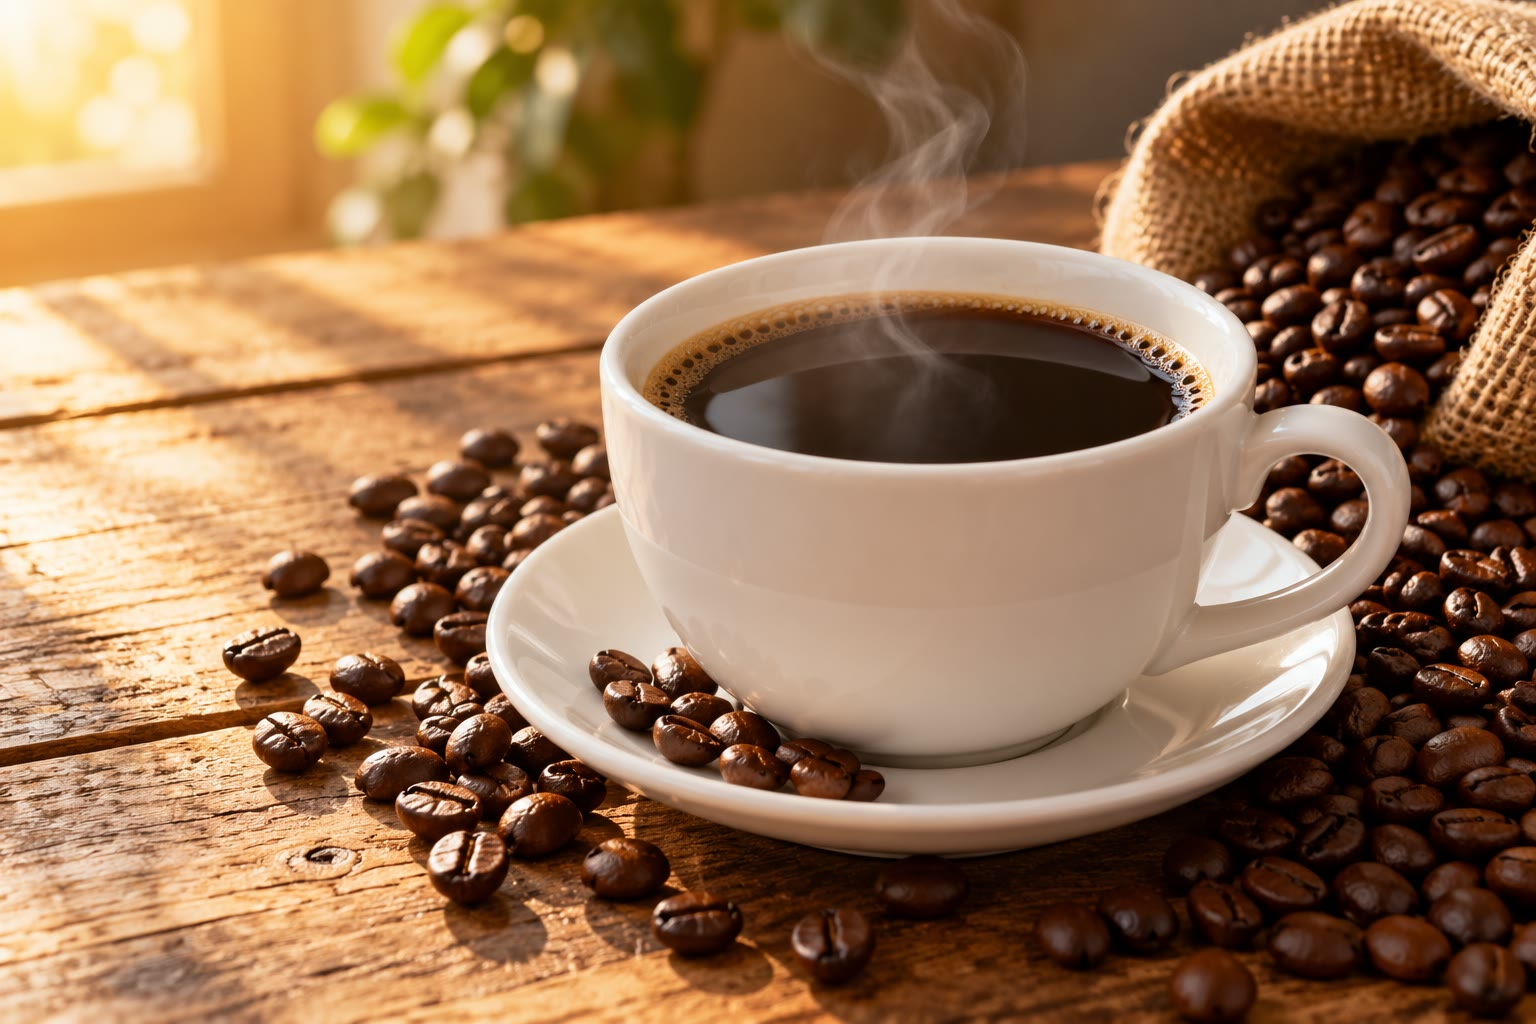
\includegraphics[width=0.5\linewidth]{images/book4/ai/b3-29-coffee.jpg}

{\small Een kop koffie en gebrande bonen: cafeïne, een purine, en veel van
de aromamoleculen die bij het branden ontstaan, zijn \omterm{def:b3:heterocycles:heterocycle}{heterocycli}.}
\end{omfigure}

\section{Aromatische heterocycli}

\begin{definition}[Heterocycli]\label{def:b3:heterocycles:heterocycle}
Een \emph{heterocyclus}\index{heterocyclus} is een ringverbinding met
minstens één ander atoom dan koolstof in de ring; een
\emph{heteroaromatische verbinding}\index{heteroaromatische verbinding} is
een aromatische heterocyclus, zoals pyridine, pyrrool, furaan of
thiofeen.
\end{definition}

\begin{proposition}[Zes $\pi$-elektronen]\label{prop:b3:heterocycles:sextet}
Pyridine, pyrrool, furaan, thiofeen en imidazool hebben elk zes $\pi$-elektronen in
een vlakke, cyclische, geconjugeerde ring, en zijn aromatisch volgens de
regel van Hückel.
\end{proposition}

\begin{proof}
Pyridine: vijf koolstofatomen en het stikstofatoom geven elk één
elektron p; het vrije elektronenpaar van stikstof zit in een $sp^2$-orbitaal in het vlak van de ring, buiten het $\pi$-systeem: $5 + 1 = 6$.
Pyrrool: vier koolstofatomen geven er elk één en het stikstofatoom,
gebonden aan H in het vlak, plaatst zijn vrije elektronenpaar in zijn orbitaal p: $4 + 2 = 6$. Furaan en thiofeen: zoals pyrrool, waarbij het
heteroatoom een van zijn twee vrije elektronenparen geeft (het andere
ligt in het vlak). Imidazool:
het stikstofatoom N--H geeft er twee, het pyridineachtige stikstofatoom
één, de drie koolstofatomen drie: 6. Zes is $4n + 2$ met $n = 1$.
\end{proof}

\begin{omfigure}
\begin{tikzpicture}[font=\small, yscale=0.55]
  % pyridine: six p orbitals perpendicular to the ring (drawn first), N at 0 deg
  \foreach \a in {0,60,...,300} { \pic at (\a:1.1) {omp={0.62}{90}}; }
  \draw[thick] (0:1.1) -- (60:1.1) -- (120:1.1) -- (180:1.1) -- (240:1.1) -- (300:1.1) -- cycle;
  \node[fill=white, inner sep=0.5pt] at (0:1.1) {N};
  \pic at ($(0:1.1)+(0.2,0)$) {omlobe={0.8}{0}};
  \node[font=\scriptsize, align=center, anchor=north] at (0,-2.4) {pyridine: 6 elektronen p van 6 atomen;\\ vrij elektronenpaar in het vlak (basisch)};
  \begin{scope}[xshift=5.4cm]
    \foreach \a in {0,72,144,216,288} { \pic at (\a:1.0) {omp={0.62}{90}}; }
    \draw[thick] (0:1.0) -- (72:1.0) -- (144:1.0) -- (216:1.0) -- (288:1.0) -- cycle;
    \node[fill=white, inner sep=0.5pt] at (0:1.0) {N};
    \draw ($(0:1.0)+(0.18,0)$) -- (0:1.7) node[right, inner sep=0.5pt] {H};
    \node[font=\scriptsize, align=center, anchor=north] at (0,-2.4) {pyrrool: het vrije paar van N is een van\\ de 6 $\pi$-elektronen (niet basisch)};
  \end{scope}
\end{tikzpicture}

{\small De $\pi$-systemen van pyridine en pyrrool, schuin gezien: één orbitaal p per
ringatoom, loodrecht op de ring. Bij pyridine wijst het vrije
elektronenpaar van stikstof (de lob in het vlak, bij het stikstofatoom)
in het vlak van de ring naar buiten en kan het vrij een proton binden;
bij pyrrool geeft het stikstofatoom, dat in het vlak een waterstofatoom
draagt, zijn vrije elektronenpaar aan het aromatische sextet.}
\end{omfigure}

\begin{definition}[$\pi$-rijke en $\pi$-arme heterocycli]\label{def:b3:heterocycles:pi-character}
Een \emph{$\pi$-rijke heterocyclus}\index{$\pi$-rijke heterocyclus}, zoals
pyrrool, furaan of thiofeen, heeft zes $\pi$-elektronen op vijf atomen en een hogere
$\pi$-elektronendichtheid op zijn koolstofatomen dan benzeen; een
\emph{$\pi$-arme heterocyclus}\index{$\pi$-arme heterocyclus}, zoals
pyridine, heeft een elektronegatief ringatoom dat $\pi$-dichtheid van de koolstofatomen wegtrekt.
\end{definition}

\begin{proposition}[Basiciteit]\label{prop:b3:heterocycles:basicity}
Pyridine is een matige base en pyrrool bijna geen; als pyrrool in sterk
zuur geprotoneerd wordt, neemt het het proton op koolstof op, niet op
stikstof.
\end{proposition}

\begin{proof}[Beargumenteerd]
% ledger: pka:pyridinium, pka4:pyrrolium, pka4:piperidinium, pka4:imidazolium, pka4:DMAPH
Het vrije elektronenpaar van pyridine ligt buiten het $\pi$-systeem: het
protoneren ervan kost geen aromaticiteit, en pyridinium heeft $\mathrm pK_a = 5.2$; het is minder basisch dan piperidine
(het stikstofatoom van pyridinium is $sp^2$, met meer karakter s, en houdt zijn paar
steviger vast: piperidinium 11.1). Het protoneren van het stikstofatoom
van pyrrool zou zijn vrije elektronenpaar uit het sextet halen en de
aromaticiteit vernietigen; alleen zeer sterke zuren protoneren pyrrool
überhaupt, op C2, waar het kation nog wat delokalisatie behoudt
($\mathrm pK_a$ ongeveer $-4$). Imidazool heeft beide soorten stikstof: het wordt geprotoneerd op het
pyridineachtige stikstofatoom, en zijn symmetrische kation wordt door
resonantie gestabiliseerd ($\mathrm pK_a$
7.0), de reden waarom histidine in \omterm{def:b3:complex-kinetics:enzyme}{enzymen} als zuur en als base werkt.
4-(Dimethylamino)pyridine is nog basischer ($\mathrm pK_a$ 9.6): de aminogroep duwt
haar vrije elektronenpaar de ring in en naar het ringstikstofatoom.
\end{proof}

% ledger: dip:pyridine, dip4:pyrrole, dip4:furan, dip4:thiophene
De dipoolmomenten vertellen hetzelfde verhaal: pyridine (\qty{2.19}{D}) heeft zijn negatieve uiteinde
op stikstof, terwijl bij pyrrool (\qty{1.84}{D}) de donatie van het vrije paar aan de
ring het negatieve uiteinde op de ring en het positieve op stikstof legt.
Bij furaan
(\qty{0.66}{D}) en thiofeen (\qty{0.55}{D}) heffen de twee effecten, $\sigma$-onttrekking en $\pi$-donatie, elkaar
bijna op.

\begin{omfigure}
% ledger: h1:pyridine.a, h1:pyridine.g, h1:pyridine.b, h1:pyrrole.a, h1:pyrrole.b, h1:pyrrole.NH, h1:furan.a, h1:furan.b
\begin{tikzpicture}
\begin{axis}[width=0.86\linewidth, height=6.2cm, x dir=reverse, xmin=5.8, xmax=9.0, ymin=-0.1, ymax=3.6,
  axis x line=bottom, axis y line=none, xlabel={$\delta$ / ppm}, tick label style={font=\scriptsize}, label style={font=\small}]
\addplot[omDef, thick] table[x=ppm, y expr=\thisrow{y}+2.4] {figdata/out/bachelor-3-heterocycle-nmr-pyridine.dat};
\addplot[omThm, thick] table[x=ppm, y expr=\thisrow{y}+1.2] {figdata/out/bachelor-3-heterocycle-nmr-pyrrole.dat};
\addplot[omMeth, thick] table[x=ppm, y=y] {figdata/out/bachelor-3-heterocycle-nmr-furan.dat};
\node[font=\scriptsize, omDef, anchor=west] at (axis cs:7.1,3.0) {pyridine: H2/6, H4, H3/5 (2\,:\,1\,:\,2)};
\node[font=\scriptsize, omThm, anchor=west] at (axis cs:7.7,1.8) {pyrrool: NH, H2/5, H3/4};
\node[font=\scriptsize, omMeth, anchor=west] at (axis cs:7.2,0.6) {furaan: H2/5, H3/4};
\end{axis}
\end{tikzpicture}

{\small Proton-NMR van pyridine, pyrrool en furaan in deuterochloroform,
gesynthetiseerd uit gemeten verschuivingen als enkelvoudige lijnen
(koppelingen weggelaten), met oppervlakten gelijk aan het aantal
protonen. Het $\pi$-arme pyridine heeft zijn signalen H2/6 en H4
ver laagveld van dat van benzeen; het $\pi$-rijke pyrrool en furaan hebben
de meeste van hun signalen hoogveld ervan; de protonen naast het
heteroatoom zijn altijd het sterkst ontschermd.}
\end{omfigure}

\section{Pyridine}

Pyridine weerstaat elektrofiele substitutie: het elektrofiel ontmoet een
ring die armer is aan elektronen dan benzeen, en, in het zuur dat
meestal aanwezig is, een pyridiniumion waarvan de positieve lading het
afstoot. Nitrering vereist zeer krachtige omstandigheden en geeft het
3-isomeer met een laag rendement.

\begin{proposition}[Elektrofiele substitutie op C3]\label{prop:b3:heterocycles:pyridine-c3}
Elektrofiele aanval op pyridine gebeurt op C3: aanval op C2 of C4 geeft
een intermediair van Wheland waarvan een van de resonantiestructuren de
positieve lading op een stikstofatoom met maar zes elektronen eromheen
zet.
\end{proposition}

\begin{proof}
In het kation uit aanval op C2 (of C4) is de positieve lading verdeeld
over C3, C5 en N1 (of C3, C5 en N1): een resonantiestructuur met een
elektronenarm stikstofatoom met zes elektronen, zeer ongunstig voor een
elektronegatief atoom. Aanval op C3 verdeelt de lading alleen over C2, C4
en C6. Alle drie de kationen zijn minder stabiel dan dat van benzeen,
maar aanval op C3 is het minst slecht.
\end{proof}

\begin{definition}[Pyridine-N-oxide]\label{def:b3:heterocycles:n-oxide}
Een \emph{pyridine-N-oxide}\index{pyridine-N-oxide}, gemaakt door pyridine
met een peroxyzuur te oxideren, heeft een groep $\mathrm{N^+{-}O^-}$ waarvan het zuurstofatoom elektronen teruggeeft aan C2
en C4; het ondergaat elektrofiele substitutie op C4, waarna het
zuurstofatoom verwijderd wordt.
\end{definition}

\begin{definition}[Nucleofiele aromatische substitutie]\label{def:b3:heterocycles:snar}
\emph{Nucleofiele aromatische substitutie}\index{nucleofiele aromatische substitutie}
($\mathrm S_\mathrm NAr$) vervangt een uittredende groep op een elektronenarme aromatische ring
door een nucleofiel, via additie gevolgd door eliminatie. Het anionische
additie-intermediair is een
\emph{meisenheimercomplex}\index{meisenheimercomplex}.
\end{definition}

\begin{proposition}[$\mathrm S_\mathrm NAr$ op C2 en C4]\label{prop:b3:heterocycles:snar-positions}
Halogeenpyridinen ondergaan $\mathrm S_\mathrm NAr$ gemakkelijk op C2 en C4 en maar traag op C3,
omdat additie op C2 of C4 de negatieve lading op het stikstofatoom zet.
\end{proposition}

\begin{proof}
Additie op C2 maakt C2 $sp^3$ en laat vier $\pi$-elektronen plus het binnenkomende paar
verdeeld over N1, C3 en C5 (of voor C4: C3, C5 en N1): één resonantiestructuur
heeft de negatieve lading op het elektronegatieve stikstofatoom. Additie
op C3 verdeelt haar alleen over C2, C4 en C6, allemaal koolstofatomen.
\end{proof}

\begin{omfigure}
\begin{tikzpicture}[font=\small, >=Stealth]
  \draw[thick] (-0.000,-0.620) -- (0.537,-0.310) -- (0.537,0.310) -- (0.000,0.620) -- (-0.537,0.310) -- (-0.537,-0.310) -- cycle;
  \draw[thick] (0.082,-0.424) -- (0.326,-0.283);
  \draw[thick] (0.326,0.283) -- (0.082,0.424);
  \draw[thick] (-0.408,0.141) -- (-0.408,-0.141);
  \node[fill=white, inner sep=0.4pt, font=\scriptsize] at (-0.000,-0.620) {N};
  \draw (0.537,-0.310) -- (0.927,-0.535) node[right, inner sep=0.5pt, font=\scriptsize] {Cl};
  \draw[thick] (3.400,-0.620) -- (3.937,-0.310) -- (3.937,0.310) -- (3.400,0.620) -- (2.863,0.310) -- (2.863,-0.310) -- cycle;
  \draw[thick] (3.726,0.283) -- (3.482,0.424);
  \draw[thick] (2.992,0.141) -- (2.992,-0.141);
  \node[fill=white, inner sep=0.4pt, font=\scriptsize] at (3.400,-0.620) {N};
  \node[font=\scriptsize, omThm] at (3.350,-0.920) {$\ominus$};
  \draw (3.937,-0.310) -- (4.386,-0.343) node[right, inner sep=0.5pt, font=\scriptsize] {Nu};
  \draw (3.937,-0.310) -- (4.190,-0.682) node[right, inner sep=0.5pt, font=\scriptsize] {Cl};
  \draw[thick] (6.800,-0.620) -- (7.337,-0.310) -- (7.337,0.310) -- (6.800,0.620) -- (6.263,0.310) -- (6.263,-0.310) -- cycle;
  \draw[thick] (6.882,-0.424) -- (7.126,-0.283);
  \draw[thick] (7.126,0.283) -- (6.882,0.424);
  \draw[thick] (6.392,0.141) -- (6.392,-0.141);
  \node[fill=white, inner sep=0.4pt, font=\scriptsize] at (6.800,-0.620) {N};
  \draw (7.337,-0.310) -- (7.727,-0.535) node[right, inner sep=0.5pt, font=\scriptsize] {Nu};
  \draw[->, thick] (1.25,0) -- (2.35,0) node[midway, above, font=\scriptsize] {$+\,\mathrm{Nu^-}$};
  \draw[->, thick] (4.65,0) -- (5.75,0) node[midway, above, font=\scriptsize] {$-\,\ce{Cl-}$};
  \node[font=\scriptsize] at (3.4,-1.2) {meisenheimercomplex};
\end{tikzpicture}

{\small Nucleofiele substitutie van 2-chloorpyridine: het nucleofiel
addeert aan C2, wat een anionisch intermediair geeft waarvan de negatieve
lading grotendeels op het ringstikstofatoom zit (één resonantiestructuur
getekend); daarna vertrekt chloride en wordt de aromatische ring
hersteld.}
\end{omfigure}

\begin{proposition}[Additie-eliminatie]\label{prop:b3:heterocycles:snar-mechanism}
Voor een reactie $\mathrm S_\mathrm NAr$ waarvan de additiestap snelheidsbepalend is, is $v = k[\mathrm{ArX}][\mathrm{Nu^-}]$,
en is fluoride de beste uittredende halogenidegroep.
\end{proposition}

\begin{proof}[Beargumenteerd]
De snelheid is die van de bimoleculaire additie. De binding
koolstof-halogeen wordt in die stap niet verbroken; wat telt, is hoeveel
het halogeen de energie van de anionische overgangstoestand verlaagt
door elektronen te onttrekken, en fluor, het meest elektronegatief, doet
dat het sterkst: de volgorde F $>$ Cl $\approx$ Br $>$ I, omgekeerd aan die van $\mathrm S_\mathrm N2$.
\end{proof}

\begin{definition}[Chichibabinreactie]\label{def:b3:heterocycles:chichibabin}
De \emph{chichibabinreactie}\index{chichibabinreactie} is de aminering van
pyridine op C2 door natriumamide: het amide-ion addeert aan C2, en een
hydride-ion gaat verloren, als diwaterstof na reactie met het product.
\end{definition}

Pyridine en DMAP dienen ook als basen en als nucleofiele katalysatoren:
bij acyleringen met zuuranhydriden valt DMAP eerst het anhydride aan, wat
een acylpyridiniumion geeft dat zijn acylgroep veel sneller aan de
alcohol overdraagt dan het anhydride zelf. Pyridinen, bipyridinen en
fenantrolinen behoren tot de meest gebruikte liganden van de
coördinatiechemie.

\section{Vijfringen}

\begin{proposition}[Elektrofiele substitutie van pyrrool op C2]\label{prop:b3:heterocycles:pyrrole-c2}
Pyrrool, furaan en thiofeen ondergaan elektrofiele substitutie vooral op
C2, omdat het kation uit aanval op C2 drie resonantiestructuren heeft en
dat uit aanval op C3 er maar twee.
\end{proposition}

\begin{proof}
Na aanval op C2 kan de positieve lading op C3 zitten, op C5, of op
stikstof, waar ze via het vrije elektronenpaar gedeeld wordt en elk atoom
een octet behoudt (derde structuur). Na aanval op C3 kan ze alleen op C2
of op stikstof zitten: de lading is minder gedelokaliseerd (zie de
figuur).
\end{proof}

\begin{omfigure}
\begin{tikzpicture}[font=\small]
  \draw[thick] (0.000,0.620) -- (0.590,0.192) -- (0.364,-0.502) -- (-0.364,-0.502) -- (-0.590,0.192) -- cycle;
  \draw[thick] (-0.303,-0.269) -- (-0.403,0.039);
  \node[fill=white, inner sep=0.4pt, font=\scriptsize] at (0.000,0.620) {N};
  \draw (0.000,0.750) -- (0.000,1.020) node[above, inner sep=0.5pt, font=\scriptsize] {H};
  \draw (0.590,0.192) -- (0.893,0.482) node[right, inner sep=0.5pt, font=\scriptsize] {H};
  \draw (0.590,0.192) -- (1.006,0.135) node[right, inner sep=0.5pt, font=\scriptsize] {E};
  \node[font=\scriptsize, omThm] at (0.164,-0.226) {$\oplus$};
  \draw[thick] (2.600,0.620) -- (3.190,0.192) -- (2.964,-0.502) -- (2.236,-0.502) -- (2.010,0.192) -- cycle;
  \draw[thick] (2.762,-0.371) -- (2.438,-0.371);
  \node[fill=white, inner sep=0.4pt, font=\scriptsize] at (2.600,0.620) {N};
  \draw (2.600,0.750) -- (2.600,1.020) node[above, inner sep=0.5pt, font=\scriptsize] {H};
  \draw (3.190,0.192) -- (3.493,0.482) node[right, inner sep=0.5pt, font=\scriptsize] {H};
  \draw (3.190,0.192) -- (3.606,0.135) node[right, inner sep=0.5pt, font=\scriptsize] {E};
  \node[font=\scriptsize, omThm] at (2.335,0.086) {$\oplus$};
  \draw[thick] (5.200,0.620) -- (5.790,0.192) -- (5.564,-0.502) -- (4.836,-0.502) -- (4.610,0.192) -- cycle;
  \draw[thick] (5.362,-0.371) -- (5.038,-0.371);
  \draw[thick] (5.113,0.395) -- (4.851,0.205);
  \node[fill=white, inner sep=0.4pt, font=\scriptsize] at (5.200,0.620) {N};
  \draw (5.200,0.750) -- (5.200,1.020) node[above, inner sep=0.5pt, font=\scriptsize] {H};
  \draw (5.790,0.192) -- (6.093,0.482) node[right, inner sep=0.5pt, font=\scriptsize] {H};
  \draw (5.790,0.192) -- (6.206,0.135) node[right, inner sep=0.5pt, font=\scriptsize] {E};
  \node[font=\scriptsize, omThm] at (5.480,0.700) {$\oplus$};
  \draw[thick] (8.400,0.620) -- (8.990,0.192) -- (8.764,-0.502) -- (8.036,-0.502) -- (7.810,0.192) -- cycle;
  \draw[thick] (8.097,-0.269) -- (7.997,0.039);
  \node[fill=white, inner sep=0.4pt, font=\scriptsize] at (8.400,0.620) {N};
  \draw (8.400,0.750) -- (8.400,1.020) node[above, inner sep=0.5pt, font=\scriptsize] {H};
  \draw (8.764,-0.502) -- (9.135,-0.700) node[right, inner sep=0.5pt, font=\scriptsize] {H};
  \draw (8.764,-0.502) -- (8.839,-0.915) node[right, inner sep=0.5pt, font=\scriptsize] {E};
  \node[font=\scriptsize, omThm] at (8.665,0.086) {$\oplus$};
  \draw[thick] (11.000,0.620) -- (11.590,0.192) -- (11.364,-0.502) -- (10.636,-0.502) -- (10.410,0.192) -- cycle;
  \draw[thick] (10.697,-0.269) -- (10.597,0.039);
  \draw[thick] (11.087,0.395) -- (11.349,0.205);
  \node[fill=white, inner sep=0.4pt, font=\scriptsize] at (11.000,0.620) {N};
  \draw (11.000,0.750) -- (11.000,1.020) node[above, inner sep=0.5pt, font=\scriptsize] {H};
  \draw (11.364,-0.502) -- (11.735,-0.700) node[right, inner sep=0.5pt, font=\scriptsize] {H};
  \draw (11.364,-0.502) -- (11.439,-0.915) node[right, inner sep=0.5pt, font=\scriptsize] {E};
  \node[font=\scriptsize, omThm] at (11.280,0.700) {$\oplus$};
  \node[font=\scriptsize] at (2.6,-1.35) {aanval op C2: drie structuren};
  \node[font=\scriptsize] at (9.7,-1.35) {aanval op C3: twee structuren};
  \draw[black!40] (6.8,-1.2) -- (6.8,1.2);
\end{tikzpicture}

{\small Intermediairen van Wheland van pyrrool (E: het elektrofiel; $\oplus$: positieve lading).
Aanval op C2 geeft een kation met de lading op C3, op C5, of op het stikstofatoom met alle
octetten volledig; aanval op C3 alleen op C2 of op stikstof.}
\end{omfigure}

Pyrrool is ongeveer even reactief als fenol of aniline: het wordt onder
milde omstandigheden gebromeerd, genitreerd en geacyleerd, polymeriseert
in sterk zuur, en wordt op C2 geformyleerd door het reagens van Vilsmeier
uit dimethylformamide en fosforylchloride. De reactiviteit daalt in de volgorde pyrrool $>$ furaan $>$ thiofeen $>$ benzeen,
volgens de bereidheid van het heteroatoom om zijn vrije elektronenpaar te
delen. Furaan, het minst aromatisch, reageert ook als dieen in
diels-alderreacties. Sterke basen zoals butyllithium deprotoneren furaan
en thiofeen op C2, naast het heteroatoom, wat
organolithiumreagentia geeft.

\begin{method}[De aanvalsplaats op een heterocyclus voorspellen]\label{met:b3:heterocycles:site}
\begin{enumerate}
  \item Deel de ring in: $\pi$-rijk (pyrroolachtig heteroatoom) of $\pi$-arm
        (pyridineachtig stikstofatoom).
  \item Elektrofielen: op een $\pi$-rijke ring op C2 (C3 bij indool, waar aanval op C2
        de benzeenring zou verstoren); op pyridine op C3, of op C4 via het
        N-oxide.
  \item Nucleofielen: op een $\pi$-arme ring op C2 of C4, vooral met een
        uittredende groep op die plaats.
  \item Sterke basen: op de C--H naast het heteroatoom.
\end{enumerate}
\end{method}

\section{Gecondenseerde en biologische heterocycli}

Indool, een benzeen gecondenseerd met een pyrrool, reageert met
elektrofielen op C3: daar houdt het intermediair de benzeenring intact,
met de lading op het stikstofatoom. Chinoline, een benzeen gecondenseerd
met een pyridine, wordt door elektrofielen gesubstitueerd op zijn
benzeenring en door nucleofielen op C2 en C4. De nucleobasen zijn
pyrimidinen (cytosine, thymine, uracil) en purinen (adenine, guanine),
een pyrimidine gecondenseerd met een imidazool. Hun oxo- en aminovormen
(lactam- en aminetautomeren) overheersen over de hydroxy- en iminovormen,
wat het patroon van waterstofbrugdonoren en -acceptoren op elke base
vastlegt, en daarmee de basenparing.

\begin{omfigure}
\begin{tikzpicture}[font=\small]
  \node[draw, rounded corners, minimum width=1.8cm, minimum height=2.8cm, fill=omDef!8] at (0,0) {};
  \node[font=\small\bfseries] at (0,1.75) {guanine};
  \node[anchor=east] (g1) at (0.85,0.85) {C6=O};
  \node[anchor=east] (g2) at (0.85,0) {N1--H};
  \node[anchor=east] (g3) at (0.85,-0.85) {C2--N--H};
  \node[draw, rounded corners, minimum width=1.8cm, minimum height=2.8cm, fill=omThm!8] at (3.2,0) {};
  \node[font=\small\bfseries] at (3.2,1.75) {cytosine};
  \node[anchor=west] (c1) at (2.35,0.85) {H--N--C4};
  \node[anchor=west] (c2) at (2.35,0) {N3};
  \node[anchor=west] (c3) at (2.35,-0.85) {O=C2};
  \draw[omMeth, very thick, dotted] (g1.east) -- (c1.west);
  \draw[omMeth, very thick, dotted] (g2.east) -- (c2.west);
  \draw[omMeth, very thick, dotted] (g3.east) -- (c3.west);
\end{tikzpicture}

{\small Een basenpaar guanine-cytosine, schematisch: drie waterstofbruggen
(groen) tussen het carbonylzuurstofatoom van guanine en een amino-N--H van cytosine, de N1--H van
guanine en de ring-N3 van cytosine, en een amino-N--H van guanine en het
carbonylzuurstofatoom van cytosine. Adenine en thymine vormen er twee.}
\end{omfigure}

\section{Ringen maken}

\begin{definition}[Synthese van Paal-Knorr]\label{def:b3:heterocycles:paal-knorr}
De \emph{synthese van Paal-Knorr}\index{synthese van Paal-Knorr} maakt een
furaan (met zuur), een pyrrool (met een primair amine of ammoniak) of een
thiofeen (met een zwavelreagens) uit een 1,4-dicarbonylverbinding.
\end{definition}

\begin{definition}[Pyridinesynthese van Hantzsch]\label{def:b3:heterocycles:hantzsch}
De \emph{pyridinesynthese van Hantzsch}\index{pyridinesynthese van Hantzsch}
condenseert een aldehyde, twee equivalenten van een $\beta$-ketoester en ammoniak tot een
1,4-dihydropyridine, dat tot het pyridine geoxideerd kan worden.
\end{definition}

\begin{definition}[Indoolsynthese van Fischer]\label{def:b3:heterocycles:fischer-indole}
De \emph{indoolsynthese van Fischer}\index{indoolsynthese van Fischer}
verhit het fenylhydrazon van een aldehyde of keton met een zure
katalysator: het hydrazon tautomeriseert tot een eenhydrazine, dat een
\omterm{def:b3:pericyclic:families}{sigmatrope omlegging} [3,3] ondergaat; cyclisatie en verlies van
ammoniak geven het indool.
\end{definition}

\begin{omfigure}
\setchemfig{atom sep=1.8em}
\schemestart
\chemfig{*6(-=-=(-NH-[:30]N=[:-30](-[:-90]CH_3)-[:30]CH_3)-=)}
\arrow{->[$\ce{H+}$][tautomeer]}[,1.4]
\chemfig{*6(-=-=(-NH-[:30]NH-[:-30](=[:-90]CH_2)-[:30]CH_3)-=)}
\schemestop
\par\bigskip
\schemestart
\arrow{->[{[3,3]}, dan][cyclisatie, $-\ce{NH3}$]}[,2.2]
\chemfig{*6(-=*5(-=(-CH_3)-N(-H)-)-=-=)}
\schemestop

{\small De \omterm{def:b3:heterocycles:fischer-indole}{indoolsynthese van Fischer} uit acetonfenylhydrazon. Zuur zet
het hydrazon om in zijn eenhydrazinetautomeer; de omlegging [3,3] breekt de
binding N--N en vormt een binding C--C tussen het ringkoolstofatoom \textit{ortho} ten opzichte van stikstof en de
eindstandige $\ce{CH2}$; het nieuwe amine valt het imine aan, en het
verlies van ammoniak geeft 2-methylindool.}
\end{omfigure}

\begin{method}[Disconnecties van een heterocyclus]\label{met:b3:heterocycles:disconnect}
\begin{enumerate}
  \item Een 2,5-digesubstitueerd pyrrool, furaan of thiofeen: disconnecteer
        beide bindingen met het heteroatoom, terug naar een 1,4-diketon
        (Paal-Knorr).
  \item Een symmetrisch 1,4-dihydropyridine met esters op C3 en C5: terug
        naar één aldehyde, twee $\beta$-ketoesters en ammoniak (Hantzsch).
  \item Een 2,3-digesubstitueerd indool: terug naar fenylhydrazine en het
        keton
        $\mathrm{R^2CH_2COR^3}$ (Fischer).
  \item Controleer de beschikbaarheid van de stukken, daarna de
        regiochemie als het keton niet symmetrisch is.
\end{enumerate}
\end{method}

\begin{definition}[Bio-isoster]\label{def:b3:heterocycles:bioisostere}
Een \emph{bio-isoster}\index{bio-isoster} is een groep die een andere
vervangt in een geneesmiddelmolecuul met behoud van de biologische
activiteit, omdat ze een gelijkaardige grootte, vorm en verdeling van
waterstofbruggen en lading heeft, zoals een tetrazool in plaats van een
carbonzuur, of een pyridine in plaats van een benzeenring.
\end{definition}

\begin{inthelab}[Een pyrrool volgens Paal-Knorr]
Hexaan-2,5-dion, aniline en een katalytische hoeveelheid
4-tolueensulfonzuur worden onder reflux verhit in tolueen in een kolf
met een dean-starkopvanger: het gevormde water wordt als azeotroop
meegevoerd en verzamelt zich in de zijarm, wat de condensatie tot
volledigheid drijft. Wanneer er geen water meer afgescheiden wordt, wordt
de oplossing gewassen met waterige natriumwaterstofcarbonaat, gedroogd en
ingedampt, en wordt het 2,5-dimethyl-1-fenylpyrrool omgekristalliseerd.
\end{inthelab}

\begin{safety}{\ghs[0.62cm]{GHS02}\ghs[0.62cm]{GHS06}\ghs[0.62cm]{GHS07}\ghs[0.62cm]{GHS08}\ghs[0.62cm]{GHS09}}
% ledger: ghs4:pyridine, ghs4:phenylhydrazine
Pyridine: zeer ontvlambaar, schadelijk langs alle wegen, met een sterke
geur; gebruikt in een zuurkast. Fenylhydrazine: giftig langs alle wegen,
kan kanker en genetische defecten veroorzaken, beschadigt het bloed bij
herhaalde blootstelling, sensibiliserend, zeer giftig voor in het water
levende organismen; het wordt met handschoenen in een zuurkast
afgewogen, en zijn afval wordt gescheiden ingezameld.
\end{safety}

\begin{history}[Twee klassieke ringsyntheses]
Emil Fischer beschreef zijn indoolsynthese in 1883, in dezelfde jaren als
zijn werk over de suikers en de purinen; Arthur Hantzsch publiceerde zijn
pyridinesynthese in 1881. Beide worden nog gebruikt: de synthese van
Fischer voor de triptanen tegen migraine, de synthese van Hantzsch voor
de dihydropyridinecalciumkanaalblokkers die hoge bloeddruk behandelen.
\end{history}

\section{Oefeningen}

\begin{exercise}[$\star$]\label{exo:b3:heterocycles:1}
Tel de $\pi$-elektronen van oxazool, thiazool, pyrimidine en purine, en zeg welke
vrije elektronenparen tot het $\pi$-systeem behoren.
\end{exercise}

\begin{exercise}[$\star$]\label{exo:b3:heterocycles:2}
Rangschik pyridine, pyrrool, imidazool, piperidine en DMAP naar
basiciteit, met hun
$\mathrm pK_a$-waarden.
\end{exercise}

\begin{exercise}[$\star$]\label{exo:b3:heterocycles:3}
Geef het belangrijkste product van de monobromering van pyrrool, van
furaan en van indool.
\end{exercise}

\begin{exercise}[$\star$]\label{exo:b3:heterocycles:4}
Geef de producten van de reactie van Paal-Knorr van hexaan-2,5-dion met
alleen zuur, met methylamine, en met fosforpentasulfide.
\end{exercise}

\begin{exercise}[$\star\star$]\label{exo:b3:heterocycles:5}
2-Chloorpyridine reageert met natriummethoxide in methanol bij \qty{65}{\celsius}; 3-chloorpyridine
nauwelijks. Verklaar, en geef het product.
\end{exercise}

\begin{exercise}[$\star\star$]\label{exo:b3:heterocycles:6}
Geef het product van de \omterm{def:b3:heterocycles:chichibabin}{chichibabinreactie} van pyridine en teken het
additie-intermediair.
\end{exercise}

\begin{exercise}[$\star\star$]\label{exo:b3:heterocycles:7}
\omterm{def:b3:heterocycles:n-oxide}{Pyridine-N-oxide} wordt op C4 genitreerd. Verklaar met
resonantiestructuren, en zeg hoe 4-nitropyridine verkregen wordt.
\end{exercise}

\begin{exercise}[$\star\star$]\label{exo:b3:heterocycles:8}
2-Hydroxypyridine bestaat in water vooral als 2-pyridon. Teken beide
tautomeren en leg uit waarom het pyridon toch aromatisch is.
\end{exercise}

\begin{exercise}[$\star\star$]\label{exo:b3:heterocycles:9}
Geef de componenten van een synthese van Hantzsch van het
1,4-dihydropyridine met methylesters op C3 en C5, methylgroepen op C2 en
C6 en een 2-nitrofenylgroep op C4.
\end{exercise}

\begin{exercise}[$\star\star\star$]\label{exo:b3:heterocycles:10}
Butanon geeft bij de synthese van Fischer met fenylhydrazine twee
verschillende indolen. Geef beide, en zeg hoe de zuursterkte hun
verhouding verandert.
\end{exercise}

\begin{exercise}[$\star\star\star$]\label{exo:b3:heterocycles:11}
Leg uit waarom 4-fluornitrobenzeen en 2-fluorpyridine sneller met
nucleofielen reageren dan de overeenkomstige chloriden, in tegenstelling tot substraten voor $\mathrm S_\mathrm N2$.
\end{exercise}

\begin{exercise}[$\star\star\star$]\label{exo:b3:heterocycles:12}
Leg met de synthetische spectra van het hoofdstuk uit hoe je pyridine,
pyrrool en furaan uit elkaar zou houden aan de hand van hun proton-NMR,
en voorspel het spectrum van
thiofeen (verschuivingen \qty{7.33}{ppm} en \qty{7.12}{ppm}).
\end{exercise}

\section{Probleem: een indool bouwen}

\begin{problem}[{Weekendprobleem --- een indool bouwen: het fenylhydrazon
van aceton, het eenhydrazine en zijn omlegging [3,3], het verlies van
ammoniak, en de keuze tussen twee indolen met butanon}]
\label{pb:b3:heterocycles:1}
% ledger: aw:C, aw:H, aw:N, aw:O
Gegevens van het probleem: 10.0 g fenylhydrazine reageert met een
overmaat aceton, en het hydrazon wordt met zinkchloride verhit.

\medskip\noindent\textbf{Deel I --- Het hydrazon.}
\begin{enumerate}
  \item Schrijf de vorming van acetonfenylhydrazon op.
  \item Waarom is het een condensatie van het imine-type, en waarom is
        een spoor zuur nuttig?
  \item Welk stikstofatoom van fenylhydrazine valt de carbonylgroep aan,
        en waarom?
  \item Bereken de molaire massa van fenylhydrazine en de gebruikte
        hoeveelheid.
  \item Bereken de theoretische massa hydrazon.
\end{enumerate}

\medskip\noindent\textbf{Deel II --- Het eenhydrazine en de stap [3,3].}
\begin{enumerate}[resume]
  \item Teken de eenhydrazinetautomeer.
  \item Welke zes atomen vormen de cyclische overgangstoestand van de
        omlegging [3,3]?
  \item Welke binding breekt en welke vormt zich?
  \item Hoeveel elektronen nemen deel, en is de stap thermisch toegestaan?
  \item Wat doet het zinkchloride?
  \item Waarom moet de aromaticiteit van de benzeenring daarna hersteld
        worden?
\end{enumerate}

\medskip\noindent\textbf{Deel III --- De ring sluiten.}
\begin{enumerate}[resume]
  \item Welk amine valt welk koolstofatoom aan om de vijfring te sluiten?
  \item Welk klein molecuul vertrekt, en wat drijft de laatste stap?
  \item Schrijf de totaalvergelijking op, van hydrazon tot 2-methylindool.
  \item Bereken de molaire massa van 2-methylindool.
  \item Bereken de theoretische massa 2-methylindool.
  \item Waar zou 2-methylindool door een elektrofiel gesubstitueerd
        worden, en waarom?
\end{enumerate}

\medskip\noindent\textbf{Deel IV --- Butanon.}
\begin{enumerate}[resume]
  \item Teken de twee eenhydrazinen van butanonfenylhydrazon.
  \item Geef de twee indolen waartoe ze leiden.
  \item Welk eenhydrazine is sterker gesubstitueerd, en welk ontstaat in
        sterk zuur?
  \item Welk indool overheerst met een zwak zuur, en waarom?
  \item Waarom kan acetaldehydefenylhydrazon niet goed indool zelf geven?
  \item Wat betekent het regiochemische probleem voor de synthese van een
        geneesmiddel?
  \item Formuleer het resultaat: de theoretische massa 2-methylindool uit
        10.0 g fenylhydrazine.
\end{enumerate}
\end{problem}
